With our implementation done, it was time to benchmark our implementation on the cluster provided by the Department of Informatics (DI) of the NOVA University of Lisbon and evaluate the parallel performance by studying some performance metrics, such as speedup, efficiency and cost. 
\par In order to test and benchmark our solution, we implemented and used some python scripts for this effect:
\begin{itemize}
    \item \verb|TestsScriptBase.py| - is considered the base of the other scripts and contains all functions and variables necessary for the other scripts to run. The script has no effect by itself, and needs to be imported by the other scripts.
    \item \verb|Benchmark.py| - like the file name implies, is used to benchmark our solution. After the benchmark, the script will export the results metrics (mean time, speedup, efficiency, cost, etc...) to the \verb|seq.csv| and \verb|omp.csv| files, which contains the metrics about the sequential (\verb|energy_storms_seq|) and paralleled (\verb|energy_storms_omp|) programs samples metrics, respectively.
    \item \verb|RunCompare.py| - Used to test the paralleled version of the program with a specific number of threads by comparing the results with the original, sequential program. The script will run both programs once.
    \item \verb|TestFilesScript.py| - Tests all test files individually and combined (example: test all test\_02 files) in order to check the correctness of the paralleled program.     
    \item \verb|BuildPlot.py| - Produces a plot with the metrics about the \verb|Benchmark.py| results. The script imports the \verb|seq.csv| and \verb|omp.csv| files produced by the \verb|Benchmark.py| script and uses the Matplotlib python module to produce the plot.   
\end{itemize}
By default, the \verb|Benchmark.py| and \verb|TestFilesScript.py| scripts will execute the original program and the paralleled program for each number of threads 5 times (for example: the script will execute 5 times the program with 1 thread, 5 times with 2 threads, etc...).
\par We have to remark that the benchmarks on the cluster were done with the energy storms programs compiled with assertions disabled. Although assertions are a very handy tool to debug our program by testing our assumptions, they are not intended to be included on the production code, since it may cause side effects on the performance, depending on how they are implemented.
\par In order to evaluate our solution after the benchmarks, it was used the following performance metrics, taught in the Concurrency and Parallelism classes:
\begin{itemize}
    \item \textbf{SpeedUp}
            \(S(p) = \frac{\texorpdfstring{T\textsubscript{1}}{nsub}}{T\textsubscript{p}}\)\\
    \item \textbf{Efficiency}
            \(E(p) = \frac{\texorpdfstring{S\textsubscript{p}}{nsub}}{p}\)\\
    \item \textbf{Cost}
            \(C(p) = p \times T\textsubscript{p}\)\\
\end{itemize}


\begin{figure}[h]
    \centering
    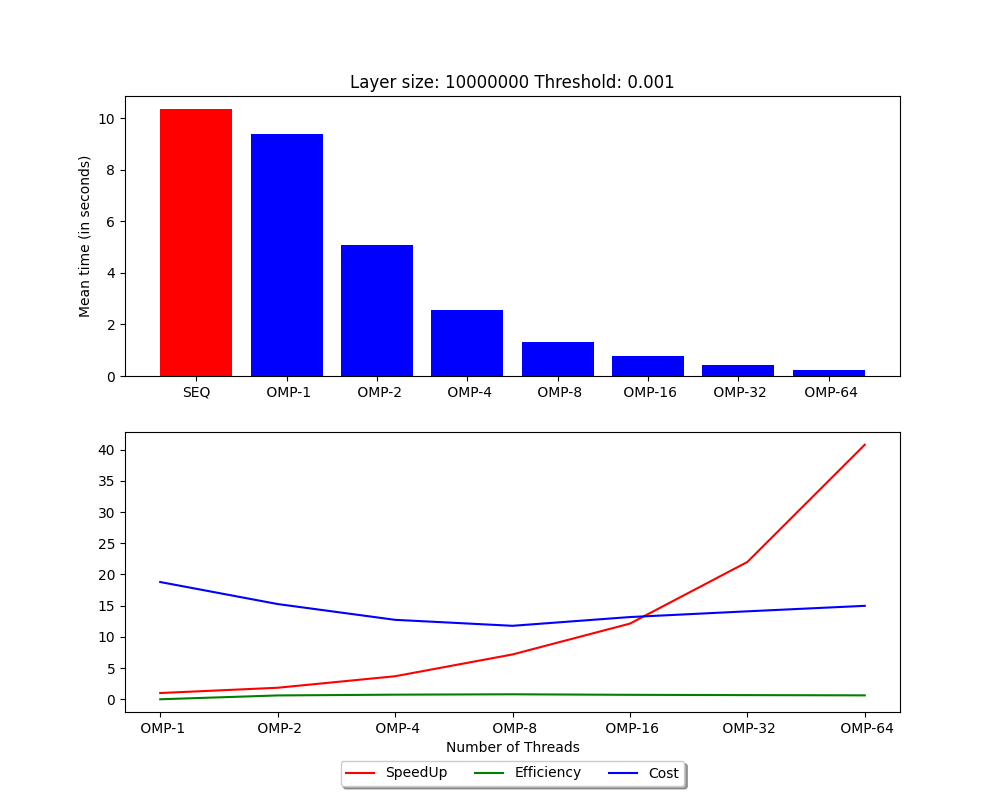
\includegraphics[scale=0.35]{images/plot_node12_all_test_01_ls_10000000.png}
    \caption{Using all test\_01 test files on node 12}
    \label{fig:my_label}
\end{figure}
\begin{figure}[h]
    \centering
    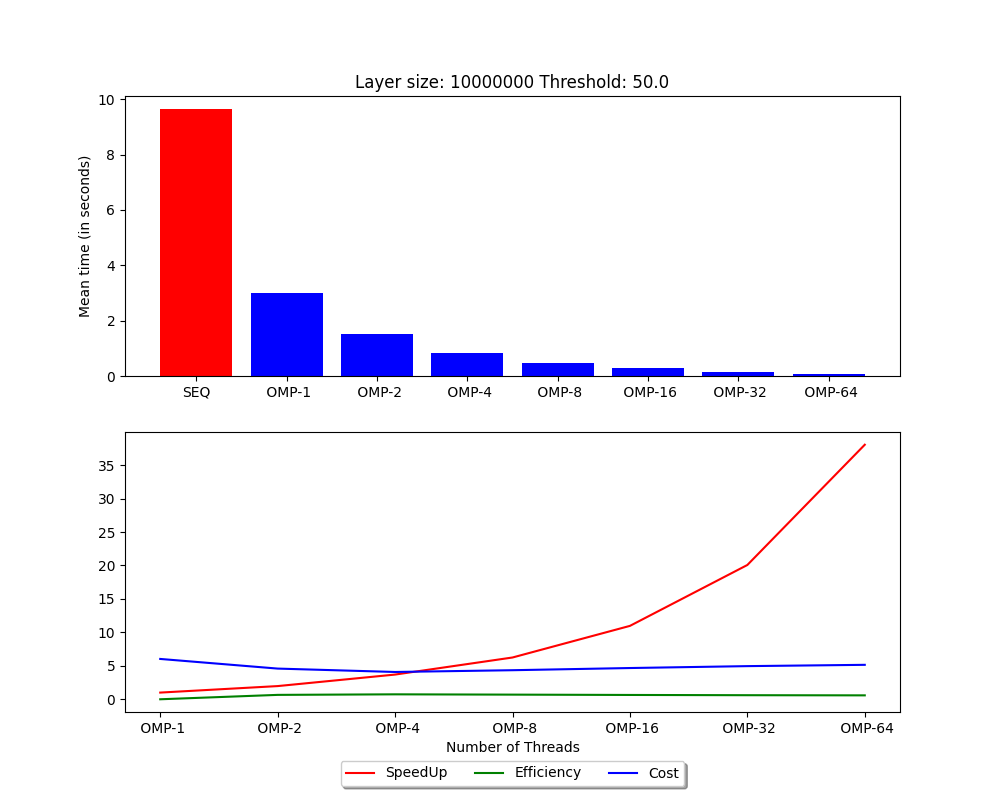
\includegraphics[scale=0.35]{images/plot_node12_all_test_01_ls_10000000_h_50.png}
    \caption{Using all test\_01 test files on node 12 with a threshold of 50}
    \label{fig:my_label}
\end{figure}
